% Created 2012-03-01 Thu 15:42
\documentclass[bigger]{beamer}
\usepackage[utf8]{inputenc}
\usepackage[T1]{fontenc}
\usepackage{fixltx2e}
\usepackage{graphicx}
\usepackage{longtable}
\usepackage{float}
\usepackage{wrapfig}
\usepackage{soul}
\usepackage{textcomp}
\usepackage{marvosym}
\usepackage{wasysym}
\usepackage{latexsym}
\usepackage{amssymb}
\usepackage{hyperref}
\tolerance=1000
\mode<beamer>{\usetheme{Madrid}}
\providecommand{\alert}[1]{\textbf{#1}}

\title{Basic Clustering}
\author{Abram Hindle}
\date{2012-02-28 Tue}

\begin{document}

\maketitle

\begin{frame}
\frametitle{Outline}
\setcounter{tocdepth}{3}
\tableofcontents
\end{frame}




\section{Introduction}
\label{sec-1}
\begin{frame}
\frametitle{What is cluster analysis?}
\label{sec-1-1}


\begin{itemize}
\item grouping objects by similar features
\item often unsupervised analysis of a dataset into ``natural'' groupings
\item explorative
\item See \href{http://en.wikipedia.org/wiki/Cluster_analysis}{http://en.wikipedia.org/wiki/Cluster\_analysis}
\end{itemize}
\end{frame}
\begin{frame}
\frametitle{Clustering}
\label{sec-1-2}


\begin{itemize}
\item Many different techniques
\begin{itemize}
\item group by
\begin{itemize}
\item connectivity
\item centroids: (the centers of a cluster)
\item distributions
\item densities
\item features
\end{itemize}
\end{itemize}
\end{itemize}
\end{frame}
\begin{frame}
\frametitle{Clustering as labelling?}
\label{sec-1-3}


\begin{itemize}
\item Single label
\begin{itemize}
\item Hierarchical clustering
\item K-means
\end{itemize}
\item Multilabel
\begin{itemize}
\item LDA
\item LSI
\end{itemize}
\end{itemize}
\end{frame}
\begin{frame}
\frametitle{Hierarchical clustering}
\label{sec-1-4}


\begin{itemize}
\item show connectivity and distance
\item partner or pair elements and then cluster these pairs
\item hierarchical grouping
\item the plot is called a Dendrogram
\item The distance metric matters
\item Distance Metric: Euclidean Distance
\begin{itemize}
\item $\sqrt \sum_{i=1}^n (p_i - q_i)^2$
\item $\sqrt p \cdot p$
\end{itemize}
\end{itemize}
\end{frame}
\begin{frame}
\frametitle{Hierarchical Clustering Dendrogram:}
\label{sec-1-5}

   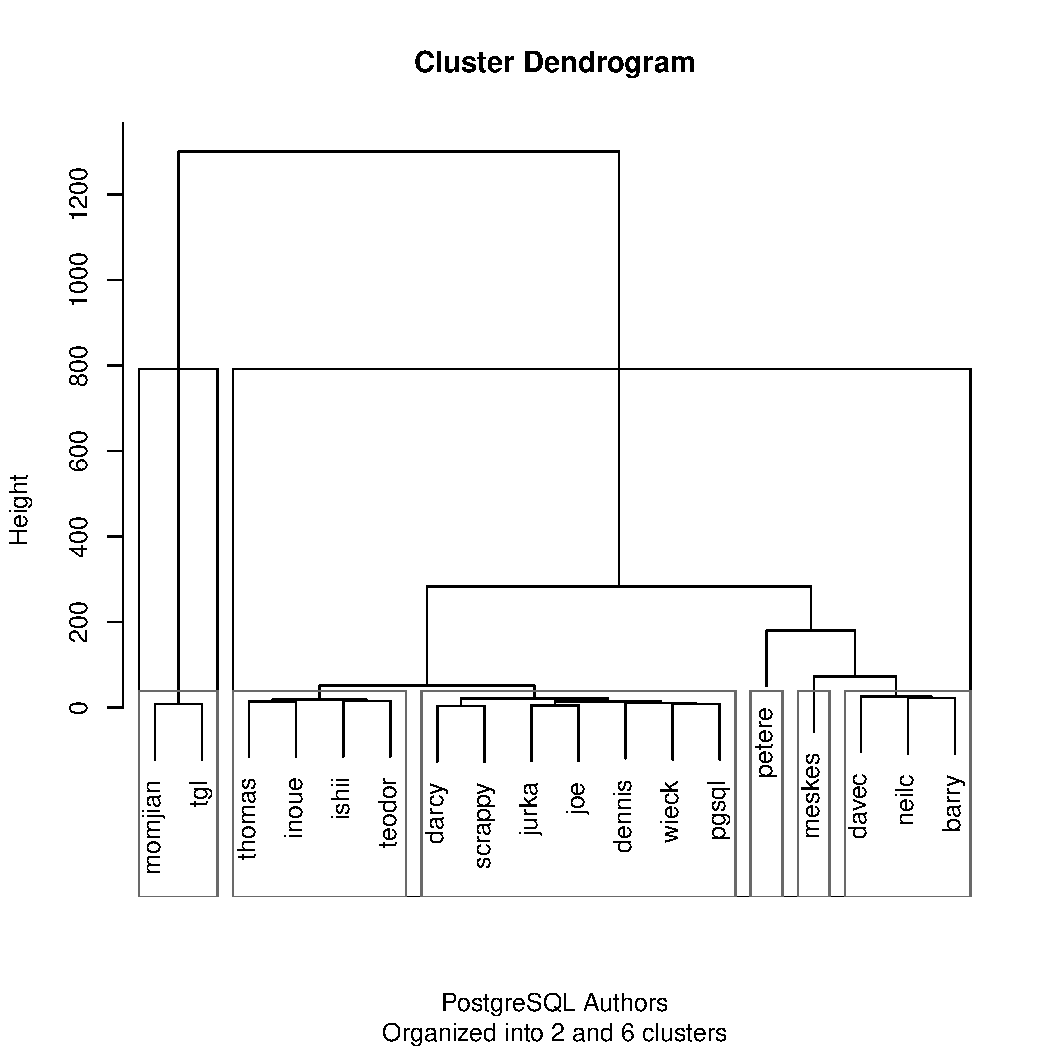
\includegraphics[height=0.8\textheight]{./postgresql-author-cluster.pdf}        
\end{frame}
\begin{frame}[fragile]
\frametitle{R code}
\label{sec-1-6}


\begin{verbatim}
v <- read.csv("Author_NFRs.csv"); vv <- v[1:18,]
for (i in 2:17) { vv[,i] <- as.numeric(vv[,i]) }
tv <- t(vv[,2:8])
authors <- matrix(tv,nrow=7,
             dimnames=list(labels(tv)[[1]],vv[,1]))
pdf("postgresql-author-cluster.pdf")
hc <- hclust(dist(t(authors)),method="ward")
plot(hc,sub="Organized into 2 and 6 clusters",
  xlab="PostgreSQL Authors")
rect.hclust(hc,k=2,border="black")
rect.hclust(hc,k=6,border="dimgrey")
dev.off()
\end{verbatim}
\end{frame}
\begin{frame}
\frametitle{Distance Functions}
\label{sec-1-7}


\begin{itemize}
\item Magnitude (Size)
\begin{itemize}
\item Euclidean  $\sqrt p \cdot p$
\item More so about size in space
\item Less concerned about membership
\end{itemize}
\item Angular (Proportional)
\begin{itemize}
\item Cosine $1 - \frac{A \cdot B}{\|A\|\|B\|}$
\item Correlation - $1 - cor(A,B)$
\item These methods are about content
\item Popular in IR
\end{itemize}
\end{itemize}
\end{frame}
\begin{frame}[fragile]
\frametitle{R code: Pearson Similarity/Distance}
\label{sec-1-8}


\begin{verbatim}
pdf("oldpostgresql-author-cluster.pdf")
hc <- hclust(as.dist(1-cor(authors)),method="ward")
plot(hc,sub="Organized into 2 and 6 clusters",xlab="PostgreSQL Authors")
rect.hclust(hc,k=2,border="blue")
rect.hclust(hc,k=6,border="purple")
dev.off()
\end{verbatim}
\end{frame}
\begin{frame}
\frametitle{Hierarchical Clustering Dendrogram: Pearson Distance}
\label{sec-1-9}

   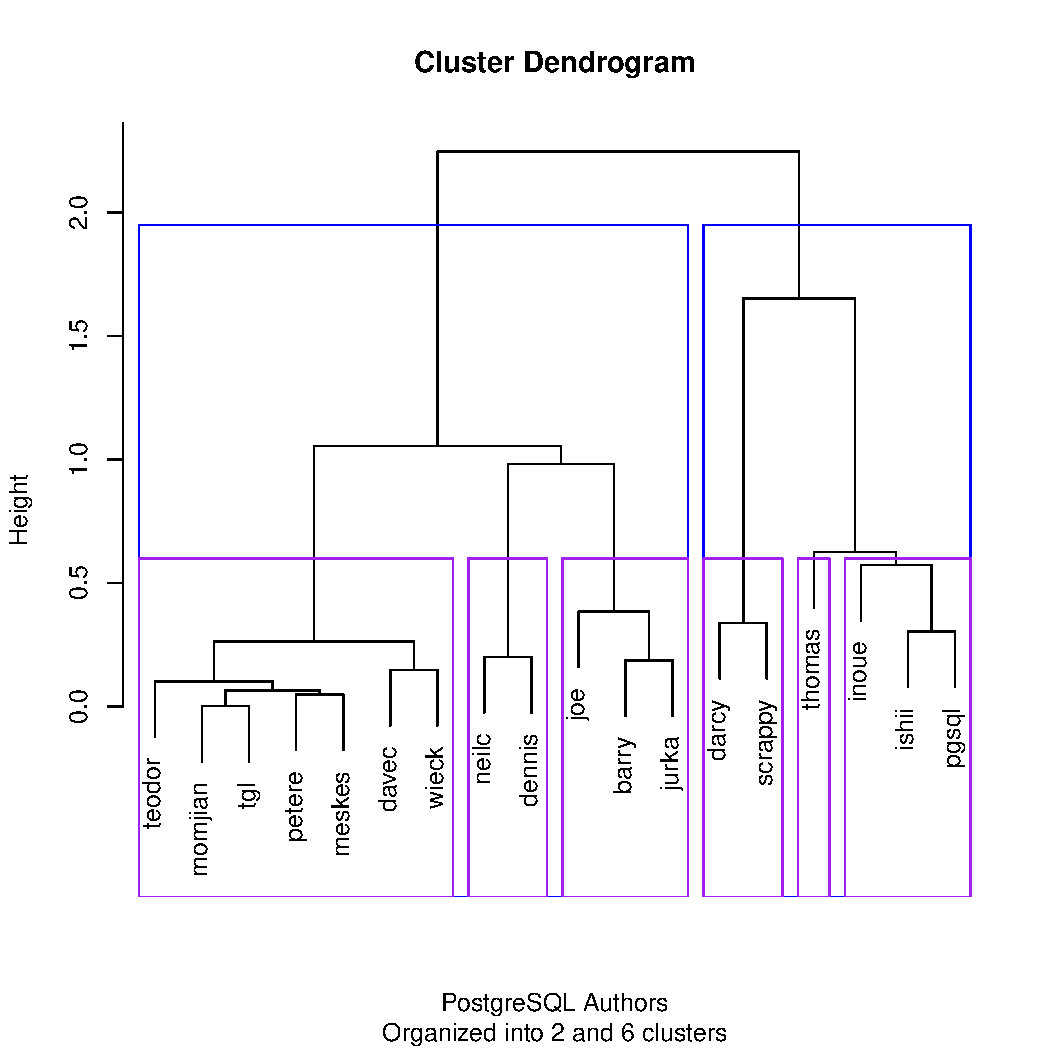
\includegraphics[height=0.8\textheight]{./oldpostgresql-author-cluster.pdf}        
\end{frame}
\begin{frame}[fragile]
\frametitle{R code: Cosine Distance}
\label{sec-1-10}


\begin{verbatim}
library(lsa)
pdf("postgresql-author-cluster-cosine.pdf")
hc <- hclust(as.dist(1-cosine(authors)),method="ward")
plot(hc,sub="Organized into 2 and 6 clusters",xlab="PostgreSQL Authors")
rect.hclust(hc,k=2,border="blue")
rect.hclust(hc,k=6,border="purple")
dev.off()
\end{verbatim}
\end{frame}
\begin{frame}
\frametitle{Hierarchical Clustering Dendrogram: Cosine Distance}
\label{sec-1-11}

   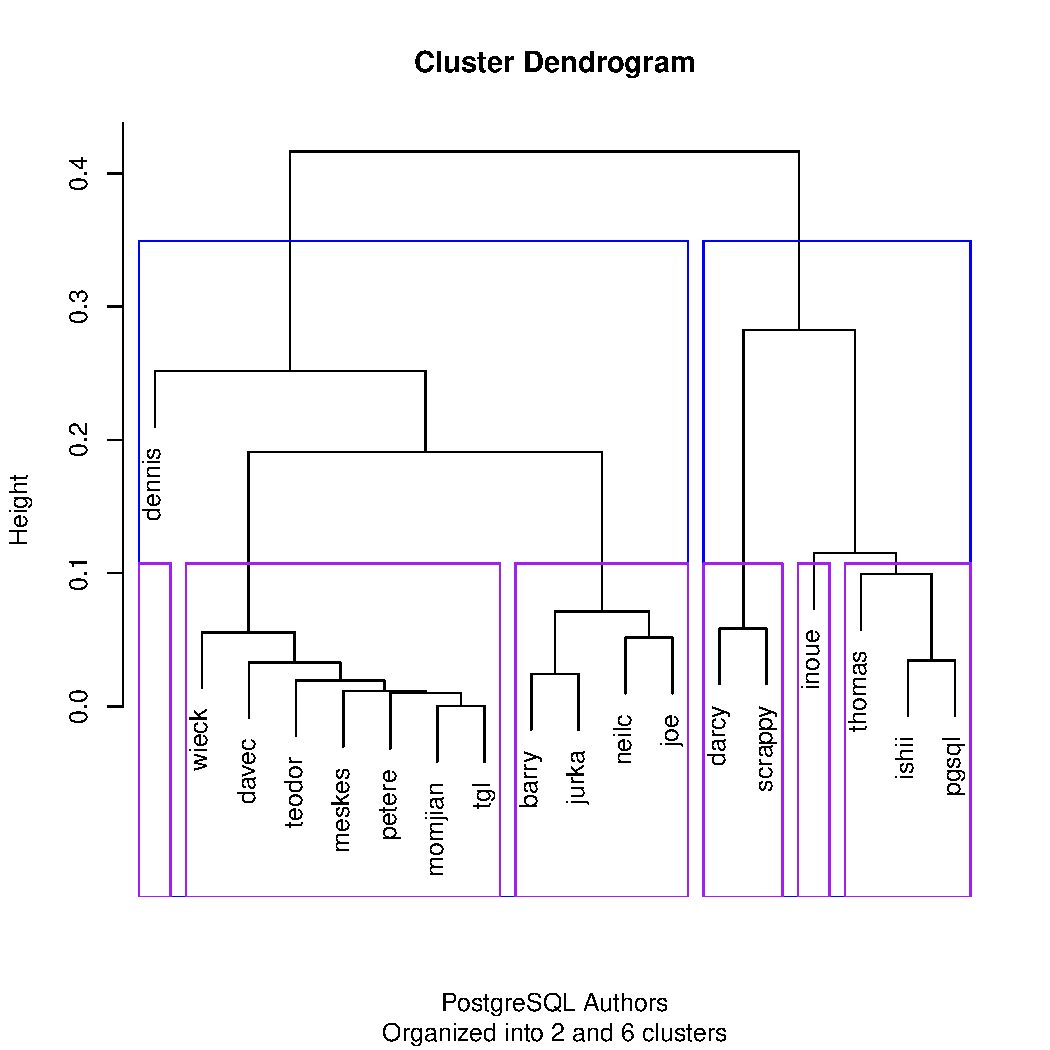
\includegraphics[height=0.8\textheight]{./postgresql-author-cluster-cosine.pdf}        
\end{frame}
\begin{frame}
\frametitle{Other Clustering Methods}
\label{sec-1-12}


\begin{itemize}
\item KMeans
\begin{itemize}
\item centroid based
\end{itemize}
\item DBScan
\begin{itemize}
\item density based
\end{itemize}
\end{itemize}
\end{frame}
\section{DBScan}
\label{sec-2}
\begin{frame}
\frametitle{DBScan}
\label{sec-2-1}


\begin{itemize}
\item Give each point a radius and then join points who's radius's
     touch.
\item Good for clusters that aren't linearly separable.
\end{itemize}
\end{frame}
\begin{frame}
\frametitle{DBScan in R}
\label{sec-2-2}


\begin{itemize}
\item in R library(fpc) has dbscan
\item data.ds = dbscan(data, 0.5)
\begin{itemize}
\item epsilon distance of 0.5
\begin{itemize}
\item warning R's dbscan is slow $O(N^2)$
\end{itemize}
\end{itemize}
\item data.ds\$cluster gives the cluster ID of the element
\end{itemize}
\end{frame}
\begin{frame}
\frametitle{DBScan in R}
\label{sec-2-3}


\begin{itemize}
\item see dbscan.R
\end{itemize}
\end{frame}
\section{KMeans}
\label{sec-3}
\begin{frame}
\frametitle{KMeans}
\label{sec-3-1}


\begin{itemize}
\item Finds K centroids
\item reliable and people understand it.
\item easy to call in kmeans(data,n) (n is the number of centroids/clusters)
\end{itemize}
\end{frame}
\section{Evaluation}
\label{sec-4}
\begin{frame}
\frametitle{Cluster Stats in R!}
\label{sec-4-1}


\begin{itemize}
\item library(fpc)
\item cluster.stats computes
\begin{itemize}
\item cluster sizes
\item diameters
\item average distance within and between clusters
\item cluster seperation
\item etc.
\end{itemize}
\item see help(cluster.stats) for references on how to use these tools
\end{itemize}
\end{frame}
\begin{frame}
\frametitle{Cluster Stats in R}
\label{sec-4-2}


\begin{itemize}
\item cluster.stats(distanceMatrix, clustering1)
\begin{itemize}
\item cluster stats of 1 clustering
\end{itemize}
\item cluster.stats(distanceMatrix, clustering1, cluster2)
\begin{itemize}
\item compare clusterings
\end{itemize}
\item see dbscan.R again
\end{itemize}
\end{frame}

\end{document}
